% \documentclass[letterpaper, twocolumn]{article}
\documentclass[sigconf]{acmart}


\usepackage{algorithm}
\usepackage{algpseudocode}
\usepackage{graphicx} 	% 1
\usepackage{wrapfig}
\usepackage{float} 		% to force figure placement
\usepackage{caption}
\usepackage{subcaption} % for the subfigure
\usepackage{amsmath} 	% to use \text{} command in math environment instead of \textrm{}
\usepackage{xcolor}
\usepackage{soul}       % for highlighting
\usepackage{xspace}
\usepackage{siunitx}
\usepackage[inline]{enumitem}
\usepackage{tikz}
\usepackage{enumitem}
%%%% Control the packages behavior
%\graphicspath{{../figures/}}

%\usepackage{booktabs} % For formal tables
%\usepackage{amsmath}
%\usepackage{hyperref}
%\usepackage{amssymb}
%\usepackage{tikz}
%\usepackage{pgfplots}
%\usepackage{lipsum}
%\usepackage{siunitx}
%\usepackage{subfig}
%\usepackage{flushend}
%\usepackage{libertine}
%\setlist{itemjoin ={,\enspace},itemjoin* = { and\enspace}}


%% New command for TODOs
\newcommand{\todo}[1]{}
\renewcommand{\todo}[1]{{\color{red} [{#1}]}}
\newcommand{\checkit}[1]{\textcolor{red}{Check---} \hl{#1}} 
\newcommand{\sys}{CIS\xspace}
\newcommand{\fullsys}{Coalesced Intermittent Sensor}
%\newcommand{\fullsys}{\sys: Battery-less Distributed Microphone}
%\newcommand{\fullsys}{Distributed Batteryless Intermittent Sensors}
%\newcommand{\fullsys}{Distributed Intermittent Systems: Theory and Practice}

\begin{document}

\title{Continuous Sensing on Intermittent Power} 

%\affiliation{\institution{Delft University of Technology}}
%\email{a.y.majid@tudelft.nl}
%
%\author{Patrick Schilder}
%\affiliation{\institution{Delft University of Technology}}
%\email{PATRIC@student.tudelft.nl}
%
%\author{Przemys{\l}aw Pawe{\l}czak}
%\affiliation{\institution{Delft University of Technology}}
%\email{p.pawelczak@tudelft.nl}
%
%\renewcommand{\shortauthors}{A.Y. Majid et al.}

%for single author (just remove % characters)
% \author{
% {\rm Amjad Yousef Majid}\\
% Delft University of Technology
% \and
% {\rm Patrick Schilder}\\
% Delft University of Technology
% % copy the following lines to add more authors
% \and
% {\rm Koen Langendoen}\\
% Delft University of Technology
% } 

\author{Amjad Yousef Majid}
\email{a.y.majid@tudelft.nl}
% \orcid{1234-5678-9012}
\affiliation{%
  \institution{Delft University of Technology}
}
\author{Patrick Schilder}
\email{p.t.schilder@student.tudelft.nl}
\affiliation{%
  \institution{Delft University of Technology}
}
\author{Koen Langendoen}
\email{k.g.langendoen@tudelft.nl}
% \orcid{1234-5678-9012}
\affiliation{%
  \institution{Delft University of Technology}
}
% \author{Stephan Wong}
% \email{j.s.s.m.wong@tudelft.nl}
% % \orcid{1234-5678-9012}
% \affiliation{%
%   \institution{Delft University of Technology}
% }


%\keywords{}

\begin{abstract}
The main obstacles to achieve truly ubiquitous sensing are (i) the limitations of battery technology - batteries are short-lived, hazardous, bulky, and costly - and (ii) the unpredictability of ambient power. The latter causes sensors to operate intermittently, violating the availability requirements of many real-world applications. 
%
In this paper, we present the \textit{\fullcis} (\cis), an
intermittently-powered ``sensor'' that senses continuously! Although
a single node will frequently be off charging, a group of nodes can
--in principle-- sense 24/7 provided that their awake times are spread
apart. As communication is too expensive, we rely on inherent component
variations that induce small differences in power cycles. This basic
assumption has been verified through measurements of different nodes
and power sources. However, desynchronizing nodes is not enough.
%
An important finding is that a \cis designed for certain (minimal)
energy conditions will become synchronized when the available energy
exceeds the design point. Nodes employing a sleep mode (to extend
their availability) do wake up collectively at some event, process it,
and return to charging as the remaining energy is typically too low to
handle another event. This results in multiple responses (bad)
and missing subsequent events (worse) due to the synchronized charging.
To counter this undesired behavior we designed an algorithm to estimate the number of active neighbors and respond proportionally to an event. 
We show that when intermittent nodes randomize their responses to events, in favorable energy conditions, the \cis reduces the duplicated captured events by 50\% and increases the percentage of capturing entire bursts above 85\%. 


% The main obstacles to achieve truly ubiquitous sensing are (i) the limitations of battery technology - batteries are short-lived, hazardous, bulky, and costly - and (ii) the unpredictability of ambient power. The latter causes sensors to operate intermittently, violating the availability requirements of many real-world applications. 
% 
% In this paper, we present the \textit{\fullcis} (\cis), an intermittently powered ``sensor'' that senses continuously!
% Our key observation being that, the power cycles of energy-harvesting battery-less devices do not show correlation even when they are drawing energy from the same source, running the same application, and in close proximity.
% We challenged our observation using different real hardware and energy sources and showed that this observation holds.
% 
% Another important finding is that a \cis designed for certain (minimal) energy conditions requires no explicit spreading of awake times due to embedded randomness in the powering subsystem. However, when the available energy exceeds the design point, nodes employing a sleep mode (to extend their availability) do wake up collectively at the next event. This synchronization leads to problems as multiple responses will be generated, and -worse- subsequent events will be missed as nodes will now recharge at the same time.
% To counter this unwanted behavior we designed an algorithm to estimate the number of active neighbors and respond proportionally to an event. 
% We show that when intermittent nodes randomize their responses to events, in favorable energy conditions, the \cis reduces the duplicated captured events by 50\% and increases the percentage of capturing entire bursts above 85\%. 

\end{abstract}
%
% The code below is generated by the tool at http://dl.acm.org/ccs.cfm.
% Please copy and paste the code instead of the example below.
%
\begin{CCSXML}
<ccs2012>
 <concept>
  <concept_id>10010520.10010553.10010562</concept_id>
  <concept_desc>Computer systems organization~Embedded systems</concept_desc>
  <concept_significance>500</concept_significance>
 </concept>
 <concept>
  <concept_id>10010520.10010575.10010755</concept_id>
  <concept_desc>Computer systems organization~Redundancy</concept_desc>
  <concept_significance>300</concept_significance>
 </concept>
 <concept>
  <concept_id>10010520.10010553.10010554</concept_id>
  <concept_desc>Computer systems organization~Robotics</concept_desc>
  <concept_significance>100</concept_significance>
 </concept>
 <concept>
  <concept_id>10003033.10003083.10003095</concept_id>
  <concept_desc>Networks~Network reliability</concept_desc>
  <concept_significance>100</concept_significance>
 </concept>
</ccs2012>
\end{CCSXML}

\ccsdesc[500]{Computer systems organization~Embedded systems}
\ccsdesc[300]{Computer systems organization~Redundancy}
\ccsdesc{Computer systems organization~Robotics}
\ccsdesc[100]{Networks~Network reliability}

\keywords{ Embedded systems, Distributed intermittent computing}

\maketitle


\section{Introduction}
\label{sec:introduction}

\begin{figure}
	\centering
	\begin{subfigure}{\columnwidth}
		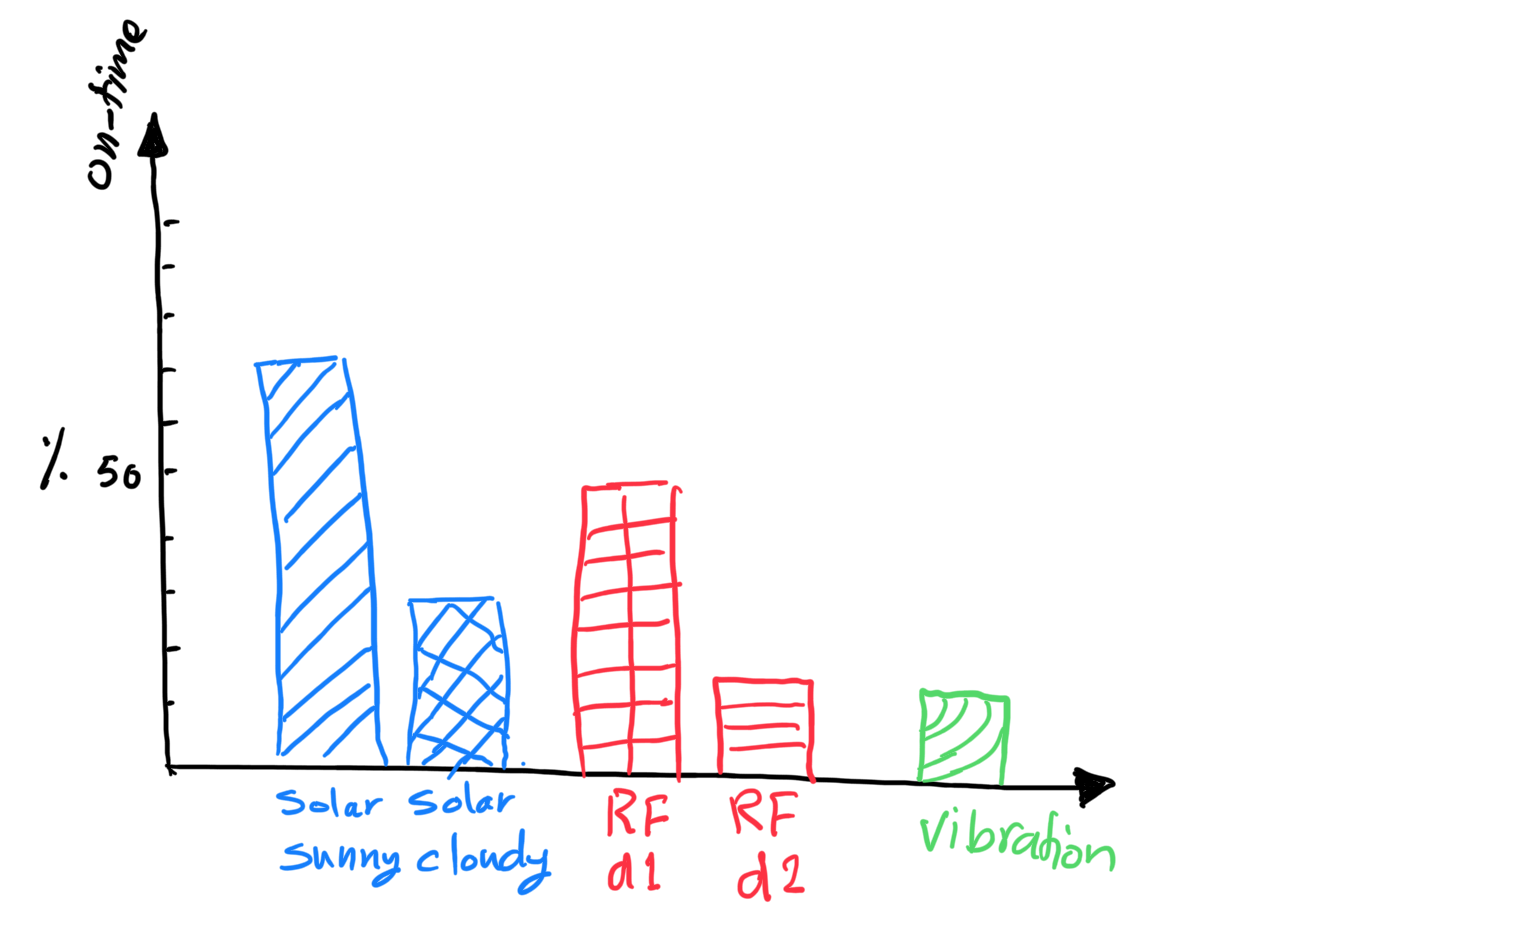
\includegraphics[width=\columnwidth]{figures/intermittent_problem}
		\caption{The on-time percentage of an intermittent device powered by different energy sources relative to its on/off cycle length}
		\label{fig:disInterSys}
	\end{subfigure}
	\begin{subfigure}{\columnwidth}
		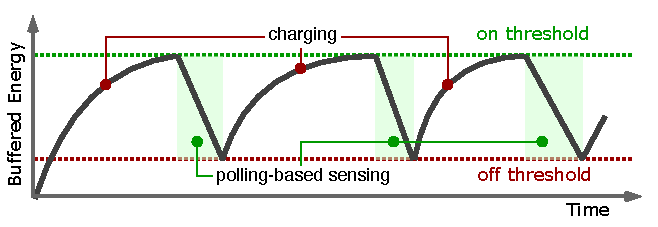
\includegraphics[width=\columnwidth]{figures/PowerCycleIntermittentSystem}
		\caption{The power cycle of an intermittently powered device.}
		\label{fig:powerCycle}
	\end{subfigure}
\end{figure}
%Intermittent software enables energy harvesting devices to run reliably despite arbitrarily timed power failures.  However, intermittent devices failed to  
%
%Self-powered tiny devices promise humanity with intelligent objects. Low cost, small size, and long operational time enable them to fundamentally change healthcare~\cite{ChenG.ISSCC2011}, water infrastructure~\cite{stoianov2007pipenet}, smart building~\cite{ardakanian2016buildsys,debruin2013monjolo}, and human-natural interaction~\cite{debruin2013monjolo}. \\
%%
%They operate by harvesting energy from ambient sources such as light~\cite{margolies_tosn_2016,margolies_infocom_2016}, vibration~\cite{gorlatova_sigmetrics_2014}, and radio frequency~\cite{rf_powered_computing_gollakota_2014} and able to compute, sense, actuate, and communicate~\cite{moo, naderiparizi_rfid_2015,flickersensys2017,smith_ubicomp_2006}.Ambient power, however, is marginal and unpredictable. Therefore,
%the execution is intermittent: it is triggered when a threshold amount of energy is buffered and terminated when the energy buffer is depleted. 

%%% Background, known information 

%An intermittently powered device (or node) starts by harvesting ambient energy. Once the harvested energy reaches a threshold, software execution begins and the energy in the buffer depletes gradually until the device shutdowns. This power cycle repeats indefinitely (Figure\,\ref{fig:powerCycle}). 

Intermittently powered devices use their environment as an energy source instead of batteries. Therefore, they promise small, cheap, and maintenance-free version of the current Internet of Things (IoT) edge devices. Driven by this vision, recent years have paid significant attention to intermittent systems~\cite{hicks2017clank,lucia2017intermittent,colin2016chain,colin2018termination,yildirim2018ink}. 
%
%%% knowledge gap, unknown information
However, their inherent sporadic operation patterns (Figure~\ref{fig:disInterSys}) have prevented researchers from demonstrating a real word applications, for example, \cite{colin2016chain,hester2017timely} present activity recognition applications without driving a real sensor to capture external signals.

%
%%% Hypothesis, question, purpose statement
This paper responds to the challenge of intermittent power supply by introducing the concept of \textit{distributed intermittent systems}. A distributed intermittent system is defined as the abstraction of a group of tiny intermittently powered devices (or nodes). The on-time of the distributed intermittent system should approach continuous time as the number of intermittent devices increases. However, the on-time and off-time of  distributed intermittent systems depend on the environment and the load. As such, we do not expect, for example, a linear relationship between the number of nodes and the overall on-time.

Controlling the on/off cycle of intermittent devices enables adapting them to many real world applications. For example, once a certain on/off cycle is preserved, an intermittent wake-up receiver can be implemented; intermittent acoustic monitoring system for monitoring engines modules---the sound produced by a deformed gear tooth---can be made. Moreover, with the advances in passive communication (such as passive light~\cite{}, and backscatter tag-to-tag~\cite{} communication) battery-free miniaturized sensors can form self-powered wireless sensor network to, for instance, create smart wallpaper and revolutionize smart buildings. 


This paper pushes the boundaries of intermittent systems by:
\todo{update the contributions and challenges}
\begin{itemize}
		\item introducing \textit{distributed intermittent systems} to control the duration of the up time of intermittent sensors and increase their responsiveness,
		\item investigating the relation between distributed intermittent systems power cycle and their environment,
		\item demonstrating the \textit{world first} distributed intermittent system: a distributed microphone. 
\end{itemize}
%\todo{add the challenges and contributions}
%%% Approach, plan of attack, proposed solution





%\section{Batteryless Distributed Sensing}
%\label{sec:disSensing}
%\subsection{Events Classification}

Given an intermittent device with a certain on-time duration ($d_{on}$), we can classify external events from the device perspective as follows:
\begin{itemize}
		\item \textit{Short events}---The event duration is shorter than the on-time of an intermittent device ($d_{on} < t_{on}$). This event can be (i) repetitive, i.e. the acoustic wave caused by a deformed gear tooth; or (ii) non-repetitive, i.e. single word command for a voice assistant.  

		\item \textit{Long events}---The event duration is much longer than the on-time of an intermittent device ($d_{on} > t_{on} $). These events can be (i) simple, such that capturing a small fraction of the event is sufficient to get all the information, i.e. vibration; or (ii) complex, such that capturing the entire event is required for correct interpretation, i.e. a command of several words to a voice assistant system. 
\end{itemize}

\subsection{Intermittent devices classifications}
Intermittent devices can be classified based on the relation between their on/off cycles and the occurrence of external events:  
\begin{itemize}
		\item An \textit{Event oblivious} intermittent device starts running once its energy buffer is full, regardless of the occurrence of an external event. In other words, the dispersion of the on-times of this type of intermittent devices is unaffected by the occurrence of external events. 
		\item An \textit{Event aware} intermittent device enters sleep mode once its buffer is full and upon the occurrence of an external event starts software execution. The power cycles of this type of intermittent devices tend to synchronize as their up times is triggered by an event.  

\end{itemize}

Events aware intermittent devices tend to have a longer effective on-time: the time needed to capture an event and save the data in memory.
%
%

%A fundamental limitation of intermittent devices are their inherent repeated absence. A natural way to combat this limitation is by grouping these tiny devices together and abstracting them as a single \emph{intermittent distributed system}. The collective on-time of these devices should approach continuous time as their number increases. However, the on-time and off-time of  distributed intermittent systems depend on the environment and the load. As such, we do not expect, for example, a linear relationship between the number of nodes and the overall on-time. 

%An intermittent device uses a capacitor (a buffer) to store energy and, usually, the capacitor has operational and shutdown thresholds (Figure\,\ref{fig:powerCycle}). 
The on-time evolution of a event-oblivious distributed intermittent system, as more nodes join, depends on the special diversity of its individual nodes.
%Depending on their spatial diversity, the nodes of a distributed intermittent system can experience the same energy harvesting conditions or not.
\subsection{Spatially Diverse Intermittent Devices}
%
\begin{figure}
	\centering
		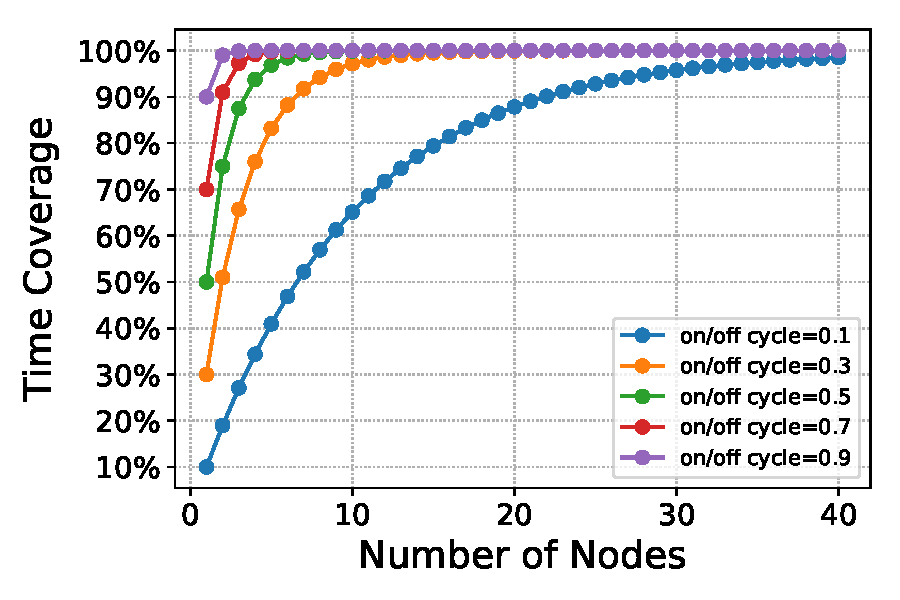
\includegraphics[width=\columnwidth]{figures/coverage.pdf}
	\caption{The on-time of a distributed intermittent system.}
	\label{fig:independentCoverage}
\end{figure}
%
\checkit{If the nodes are spatially diverse such that their energy harvesting rates are statistically different, then we can assume that the power cycles of the nodes are independent and uniformly distributed over the overall distributed system's power cycle}---When all the nodes power up and shutdown again\footnote{\todo{maybe it is better to define it as the mean of the individual power cycles}}. 
When the power cycles are uniformly distributed, adding a node increases the average on-time as follows, 
%
\begin{equation}
\delta t = \frac{t_{off}}{s_{pc}} * n_{on}
		\label{eq:indCov}
\end{equation}
%
where $t_{off}$ is the off-time of the distributed system, $s_{pc}$ is the period of the distributed system's power cycle, $n_{on}$ is a node on-time, and $\delta t$ is the time gain of the distributed intermittent system.

As Figure\,\ref{fig:independentCoverage} shows adding nodes to intermittent distributed systems increases its overall on-time, and consequently, its responsiveness. It is also clear that the benefit of an additional node is inversely proportional to the distributed system's on-time. Equation~\ref{eq:indCov}, however, holds only when nodes wake-ups approximate a uniform distribution. \checkit{When the nodes are in close proximity, we cannot model their power cycles as a random variable drawn from a uniform distribution because their energy charging rates are correlated}. 

\subsection{Spatially Invariant Intermittent Devices}
%
\begin{figure}
	\centering
	\begin{subfigure}[t]{0.49\columnwidth}
		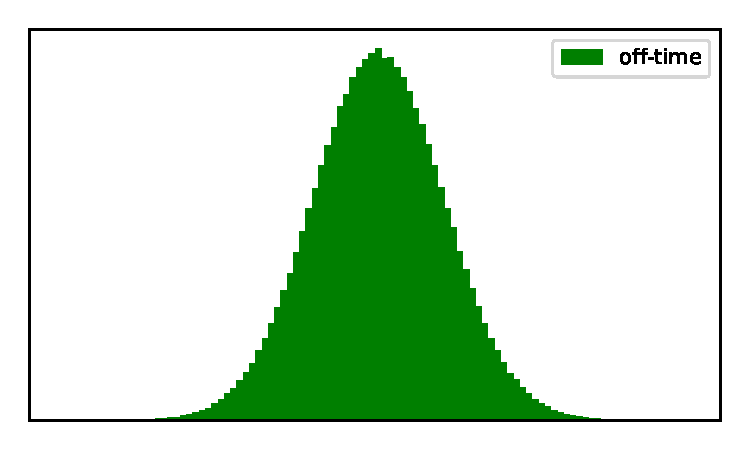
\includegraphics[width=\textwidth]{figures/offtime.pdf}
			\caption{off-time length distribution}
		\label{fig:offtime}
	\end{subfigure}
	\begin{subfigure}[t]{0.49\columnwidth}
		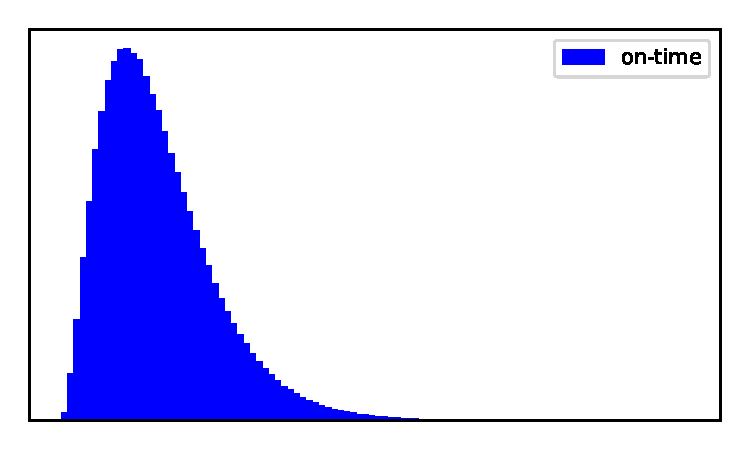
\includegraphics[width=\textwidth]{figures/ontime.pdf}
		\caption{on-time length distribution}
		\label{fig:ontime}
	\end{subfigure}
		\caption{The distributions of the operational stages of a distributed intermittent system.}		
\end{figure}
%
To understand how the on-time of a distributed intermittent system evolves when devices' power-ups are correlated, we need to investigate the \checkit{variance} of the off-time and on-time intervals.  

The \textit{off-time} of an intermittent device depends only on the environment: high charging rate results in short charging time and vice versa. Hence, we may model the off-time as a random variable drawn from a normal distribution (Figure\,\ref{fig:offtime}). The \textit{on-time}, however, depends on the buffered energy---the harvested energy while the device is off---; the harvested energy while the device is on, which only prolongs the execution; and the load of the device. Therefore, if we assume the load is constant, then we can model the on-time as a random variable drawn from a gamma distribution can be more appropriate (Figure\,\ref{fig:ontime}). Another important factor is \textit{the relation} between the off-time and the on-time. Short off-time indicates a high charging rate. A high harvesting rate results in a non-negligible amount of the harvested-while-executing energy. This energy lengthens the on-time. Therefore, we can conclude that there is an inverse relationship between the on-time and the off-time. \checkit{By considering these three factors (on-time, off-time, and their relation), we can model the variation in intermittent devices' power cycles as a normal distribution}. As a result, when charging rates are correlated, the power-ups of intermittent nodes will tend to cluster around the mean instead of spreading over the entire power cycle of the distributed intermittent system. 

\todo{relocate the following paragraph}
To flatten the normal distribution we need to add another random variable that is drawn from a uniform-like distribution. To achieve that, we further randomize the length of the on-time of intermittent nodes by injecting delays---putting the nodes into sleep mode---upon devices' power-ups (Figure\,\ref{fig:spreading}). The maximum delay that can be added is bounded by the buffer size and the minimum energy consumption of the load. The length of this delay represents the spreading factor by which we spread the original distribution of the nodes' wake-ups.  


\todo{Update equation 1 to include the spreading factor}

\begin{figure}
	\centering
		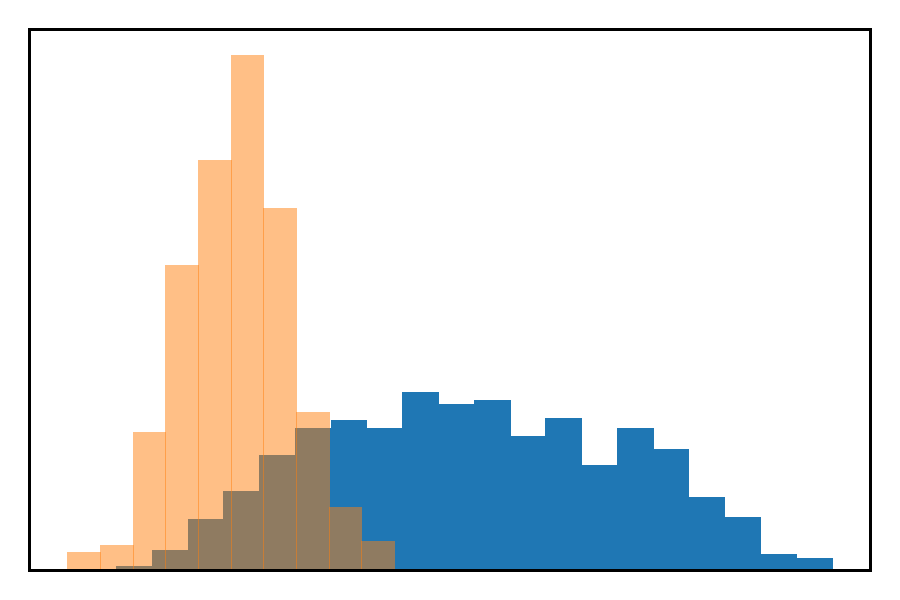
\includegraphics[width=\columnwidth]{figures/spreading.pdf}
	\caption{Spreading normally distributed intermittent devices over a larger range by injecting delays with a uniformly distributed lengths.}
	\label{fig:spreading}
\end{figure}
%The energy charging rate is environment dependent, while the discharge rate is load dependent. If we assume ambient energy does not fluctuate very quickly, then we can conclude that there is an inverse relationship between the on-time (discharging time) and the off-time (charging time). Short charging time means fast energy shots arrival. High energy harvesting rate prolongs discharge (execution) time, as the device harvests a nonible amount of energy while executing. 





















\section{Coalesced Intermittent Sensing}
\label{sec:coalInterSen}
\fullsys (\sys) is the abstraction of a group of batteryless intermittent sensors. \sys orchestrates its nodes power cycles using a distributed approach (instead of relying on a master powerful node to coordinate coalesced nodes activities). 
%\sys seeks maximum time span of its underlying coalesced nodes through a distributed approach instead of a master node that orchestrates coalesced nodes on/off cycles. 

\subsection{Intermittent Nodes' Power Cycles Distribution}
To ensure an efficient distribution of the intermittent nodes' uptimes, an explicit or implicit control methods can be applied: (i) explicit control of nodes' power cycles requires inter-nodes communication. Communication between batteryless nodes requires ultra low power communication regimes to be efficient. Recent advancements in passive visible light communication~\cite{Marco} and ambient radio frequency backscattering~\cite{} demonstrate the feasibility of extremely energy efficient communication between batteryless nodes. Once messages exchange is possible, an intermittent node duty is to estimate the number of active nodes in its time slot and to decide on leaving this power cycle of maintaining it (Figure~\ref{xxx}). Nodes can influence their power cycles by altering their load---low power consumption extends a node's uptime and delays its off-time, and high power consumption has an inverse effect. (ii) implicit control of nodes' power cycles approach seeks to use a random process to "ideally" uniformly distribute nodes' on/off cycles over the \sys's power cycle: when all the nodes complete their individual power cycles. \sys takes advantage of the randomized nature of the ambient energy to distribute its coalesced nodes. 

In this paper we opt to explore the implicit nodes distribution control approach as it is simpler and requires less overhead than explicit control methods~\footnote{The hardware used to demonstrate the feasibility of passive light communication and ambient RF backscattering are not open source and re-making it is beyond the scope of this study \todo{add the references to Marco's paper and ambient RF paper}}.


\paragraph{Implicit Control: Exploiting Solar Power}
%
The implicit control methods have the advantage of not requiring control messages exchanging and processing. 
%
\begin{figure}
	\centering
		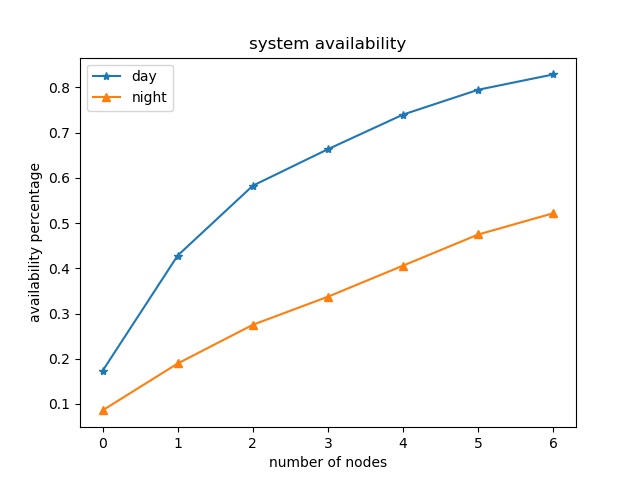
\includegraphics[width=\columnwidth]{figures/solarPoweredCoIS.png}
	\caption{Implicit \fullsys' nodes distribution using solar power harvesting randomization}
	\label{fig:solarPwrCoIS}
\end{figure} 

Figure~\ref{fig:solarPwrCoIS} shows an implicit solar power based \sys's nodes distribution when they are powered by artificial light (during night) and sunlight (during day). 





\subsection{Sensing on Intermittent Power}


%\section{Distributed Intermittent System}
\section{Batteryless Distributed Microphone}
\label{sec:disMic}
\begin{figure}
	\centering
	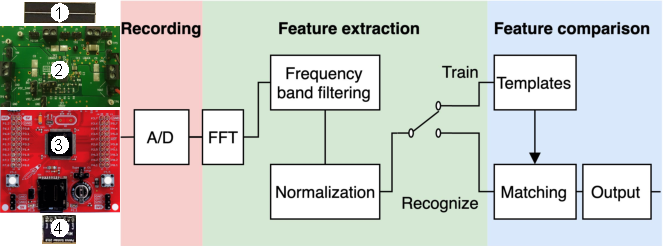
\includegraphics[width=\columnwidth]{figures/cis}
	\caption{\fullCIM: an instant of a \fullsys. \cim features a power failure immune word recognizer. Once a word is recorded, the word's spectral features extraction begins. The resulting features vector is compared against previously-stored words' templates for recognition. The comparison using a liner distance matching algorithm}
	\label{fig:cis}
\end{figure}

We have developed a prototype of a \fullcim (\cim): an instant of a \fullsys. The \cim consists of eight batteryless intermittent nodes. Each node is capable of performing isolated words recognition. 

The reason behind developing a \cim is threefold: (i) voice is a natural and convenient way for human to interact with miniaturized devices; (ii) demonstrating \textit{the world's first} batteryless intermittently-powered command recognizer, which shades light on the potential of batteryless intermittent systems; and (iii) facilitating testing with different sensing strategies and different type of external events arrival (i.e. regular  or burst). 

Moreover, we believe that a \cim can facilitate direct human-to-human or human-to-objects communication. Imagine that a \cim based system is deployed in a play ground, embedded in ground and other objects. You want to call your child, and a \cim based system is embedded in your shirt and his shirt. You say his name and the \cim picks up the word and scatter it over light---\cite{marco} demonstrates the feasibility of scattering sunlight to communicate between two nodes that are up to 60\,m apart. The scattered signal will be relied on other \cim nodes until the receiving node on his shirt receives the message and notify him, daddy is calling. 

\subsection{Hardware}
A \cim node consists of thee main parts: a microphone, a microcontroller, and a harvester. MSP430RF5994~\cite{ti_msp430_website} an ultra-low-power microcontroller is used for data acquisition and processing. This microcontroller has a 16-bit RISC processor running on 1 MHz, 8KB of SRAM (volatile), 256KB of FRAM (non-volatile), and a 12-bit analog to digital converter (ADC). It also features a Low Energy Accelerator (LEA), which offloads the main CPU for specific operations, such as FFT. For recording we use the PMM-3738-VM1010-R piezoelectric MEMS microphone, which features Wake on Sound and ZeroPower listening technologies \cite{microphone}, allowing both the microcontroller and the microphone to sleep in a low-power mode until a sound wave is detected.
The microcontroller and microphone are powered by a BQ25570 solar power harvester~\cite{BQ25570EVM-206_website} connected to an IXYS SLMD121H04L solar cell~\cite{SLMD121H04L_website} and a super-capacitor of 470 \si{\micro F}. For debugging we used the Saleae logic analyzer~\cite{saleae}.

\subsection{System Description}
The \cim has a power interrupts immune command recognizer. The recognizer is capable of recognizing isolated-word type of speech. 
The main parts of the recognizer are illustrated in Figure~\ref{fig:cis} and explained below:

\subsubsection{Data acquisition}
The \textit{Wake-on-Sound} feature of the microphone triggers the data acquisition process once the energy level in the sound signal crosses a certain level. The ADC, then, samples the output of the microphone at 7,812\,Hz. This sampling rate is sufficient to cover most of the frequency range of the human voice. To determine the end of the recording we relied on the characteristics of the targeted vocabulary. In particular, we identified, experimentally, the minimum effective recording length, which is happened be 259\,ms for the chosen set of words. By exploiting the Wake-on-Sound feature and the minimum effective recording length we eliminate the need for an endpoint detection algorithm~\cite{}, greatly improving the processing time and system efficiency from the energy perspective.


\subsubsection{Feature Extraction}
Once a recording has finished, framing and data processing begin. \cim divides the digitized signal into non-overlapping frames of 256 samples ($\approx$ 33 milliseconds). This size is beneficial for doing a Fast Fourier Transform and short enough for the voice-features to be considered constant inside a frame.

To extract the spectral features of a frame, \cim divides the frequency of interest into 12 bands (as in~\cite{hopper1992}). The first five bands has a bandwidth of 200\,Hz. The next three has a bandwidth of 300\,Hz which is followed by two bands of 500\,Hzs. Finally, the last two bands has a 600\,Hz bandwidth. This division is motivated by how the energy is concentrated in human speech~\cite{hopper1992}. Then, \cim computes the 256-point Fast Fourier Transform for each frame. The resulting feature vector contains the amount of energy concentrated in each frequency band defined earlier. This feature vector forms the basis for the words identifying process once it is normalized.

Normalization minimizing detection errors that result from differences in the amplitude of the speech input of a word. To normalize a feature vector, \cim computes the binary algorithm of each entry of that vector. 
Then it computes the mean of the resulting vector. Finally, it subtracts each entry of the resulting vector from the computed mean. This is summarized in the following equation: 
\begin{equation}
    f_i = \log(\hat{f}_i) - \frac{\sum\limits^S_{i=1}\log(\hat{f}_i)}{S},
\end{equation}
where $f_i$ is the normalized output for the $i^{\text{\tiny th}}$ spectral band of a feature vector, $\hat{f}_i$ is the energy in the $i^{\text{\tiny th}}$ spectral band of the frame, and $S$ is the number of spectral bands (12 in our case). 

\subsubsection{Feature Matching}
Feature matching is done by computing the distances between the normalized feature vectors of the recorded word and the vectors of the words stored during the training phase. 
\cim computes the squared Euclidean distance between vectors as follows,
\begin{equation}
	 	d_j = \sum\limits^S_{i=1} (f_{s,i} - f_{r,i})^2,
    \label{eq:frame_dist}
\end{equation}
where $d_j$ is the distance between the $j^{\text{\tiny th}}$ stored and recorded vectors. $f_{s,i}$ is the normalized output of the $i^{\text{\tiny th}}$ spectral band of a stored vector, $f_{r,i}$ is the normalized output of the $i^{\text{\tiny th}}$ spectral band of a recorded vector. 
The total distance between two words is calculated as follows:
\begin{equation}
		D_k = \sum\limits^{l}_{j=1} d(j)
\end{equation}
where $D_k$ is the distance between the $k^{\text{\tiny th}}$ stored word and the recorded word, and $l$ is the recording length measured in frames.

Once the recorded word has been compared to all \cim dictionary words, the word with the smallest distance to the recorded word is considered the correct word. However, if the smallest distance is bigger the garbage threshold \todo{Partick uses confusion matrix for setting this threshold. Maybe I need to consider adding it} which we experimentally set, then the \cim will return "undefined word". 

It should be emphasized that in Linear distance matching (LDM) the feature vectors of two words are compared successively, not accounting for differences in pronunciation speed. This is sufficient for our case as we are targeting isolated words and speaker dependent speech recognition type\footnote{We have also implemented Dynamic Time Warping algorithm which better handles the difference in the speed of speech. However, it is slower than the linear matching algorithm and the detection accuracy were comparable in our case}. 

\subsubsection{Power Failure Protection}
In order to preserve the progress state and to protect \cim data against randomly timed power failures, we manually splitted \cim program into 19 atomic regions. We ensured the each of these regions requires less energy the what the energy buffer can provide with a single charge. The program progress state is saved in the non-volatile memory (FRAM) on the transition between these regions. This prevents the program from falling back to its starting point (\texttt{mian()}) after each power failure. Data in the non-volatile memory with Write-After-Read dependency are double buffered to ensure the data integrity when the power supply is interrupted. 

\subsection{Code profiling}
The entire command recognition software was written in the {\tt C} programming language. The total program consists of 973 lines of code, excluding the Texas Instrument DSP library, from which the FFT function was used. See \ref{tab:code_stats} for more information.

The memory footprint on the microcontroller was 20,064 bytes of FRAM and 1,134 bytes of SRAM. Execution times are shown in \ref{tab:profiling}.

The power usage of a node differs according to it's activity. When a node is waiting for a voice event, it is in low-power mode. When data needs to be processed or recorded it is in active mode. When recording, the microphone and ADC consume additional power. The power consumption rates are measured with a Monsoon power monitor~\cite{monsoon} and shown in \ref{tab:power_usage}.


\begin{table}
	\centering
	\caption{Code statistics: lines of code}
	\label{tab:code_stats}
	%Compiled without optimization flags:
	\begin{tabular}{lrrrr} \hline
		Language & Files & Blank & Comment & Code \\\hline
		C & 7 & 264 & 173 & 736 \\
		C/C++ Header & 8 & 62 & 40 & 237 \\\hline
		Total &  15 & 326 & 213 & 973 \\\hline
	\end{tabular}
\end{table}

\begin{table}
	\centering
	\caption{Power usage.}
	\label{tab:power_usage}
	%Compiled without optimization flags:
	\begin{tabular}{lrrr}\hline
	Section & Current (\si{\micro A}) & Voltage (V) &  Power (\si{\micro W}) \\\hline
	Sleeping & 64 $\pm$20 & 2.008 $\pm$? & 128 $\pm$40 \\
	Recording & 423 $\pm$20  & 2.008 $\pm$? &  849 $\pm$40\\
	Processing &  282 $\pm$20 & 2.008 $\pm$?& 566 $\pm$40 \\\hline
	\end{tabular}
\end{table}

\clearpage


\section{Evaluation}
\label{sec:evaluation}
\begin{figure*}[h]
        \begin{subfigure}{.66\columnwidth}
            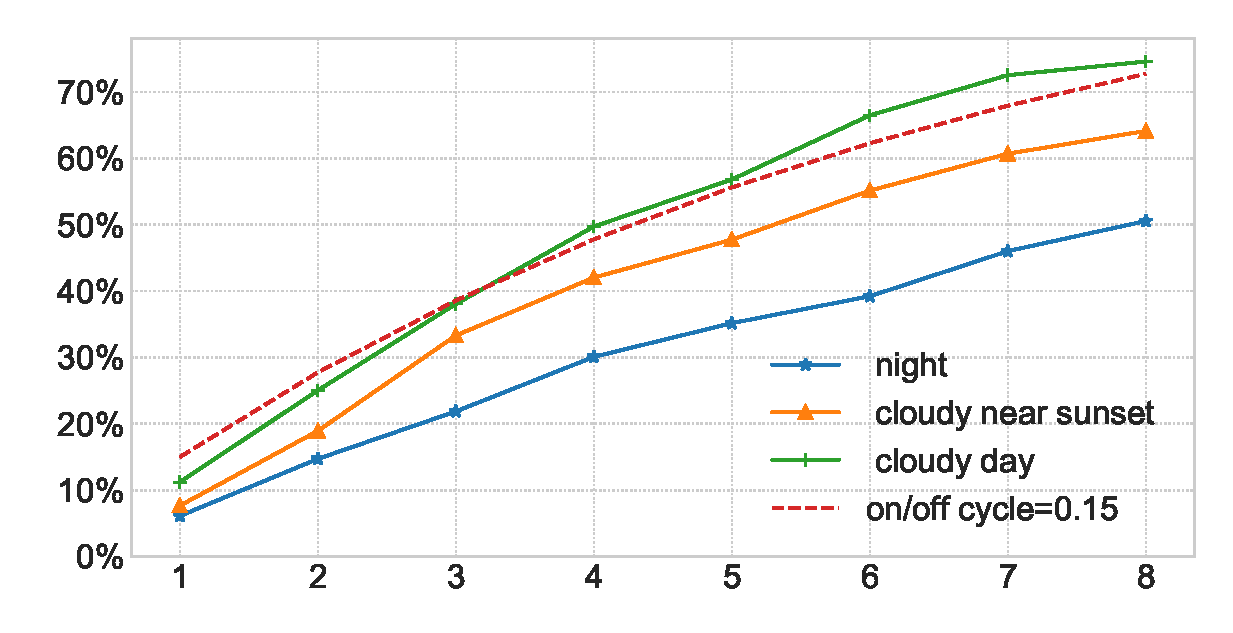
\includegraphics[width=\textwidth]{figures/sysAvailability}
                \caption{The \cis is powered by uncontrollable light sources---artificial light (night) and sunlight (day).}
            \label{fig:solarPwrCIS}
        \end{subfigure}\hfill
        \begin{subfigure}{.66\columnwidth}
            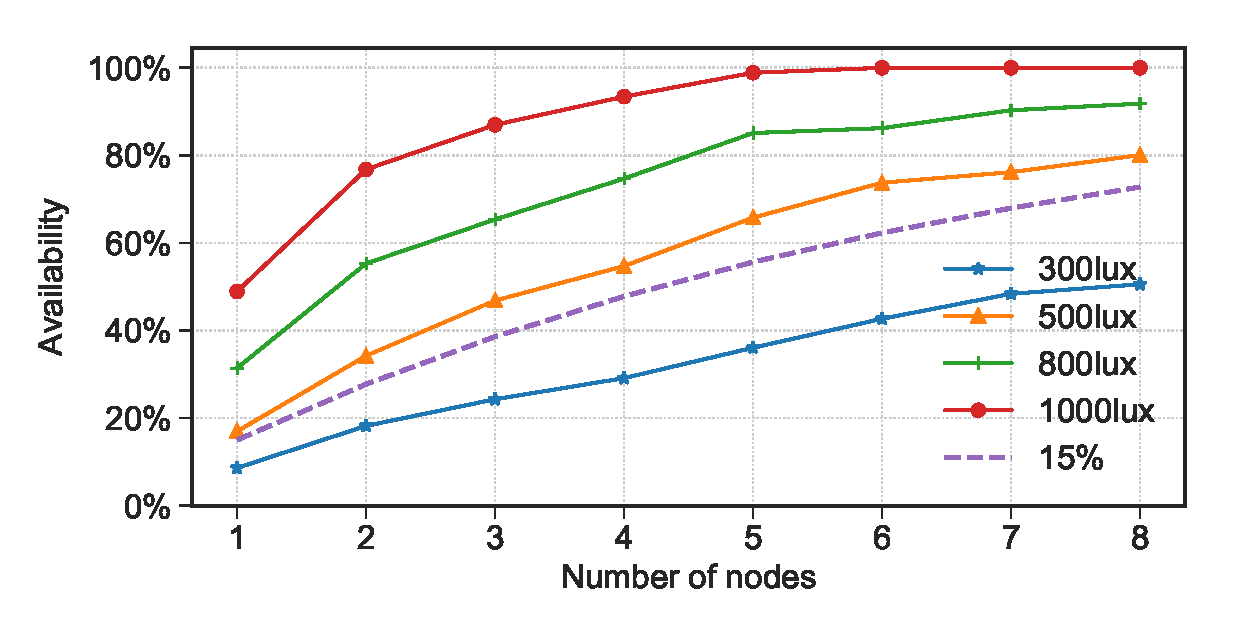
\includegraphics[width=\textwidth]{figures/sysAvailability_artificial-light}
                \caption{The \cis is powered by a controllable array of LEDs. \vspace{1em}}
            \label{fig:artPwrCIS}
        \end{subfigure}\hfill
        \begin{subfigure}{.66\columnwidth}
            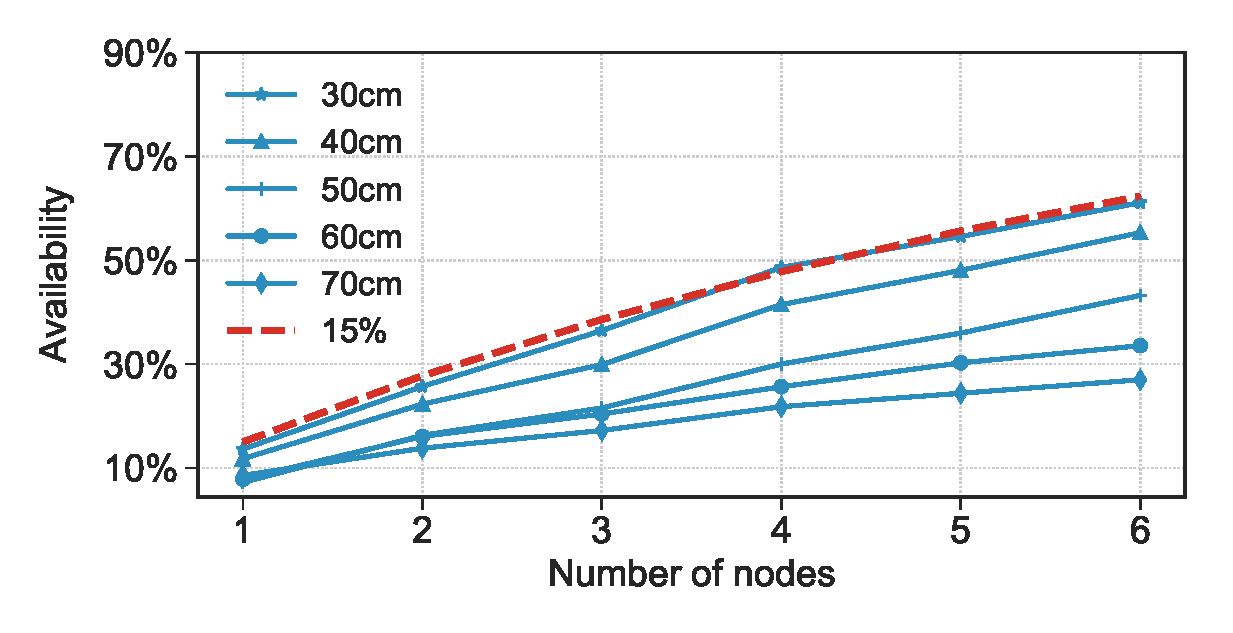
\includegraphics[width=\textwidth]{figures/rf_sysAvailability}
                \caption{The \cis is powered by an RF reader~\cite{r420_website} located 30-70\,cm away from the RF tags (WISPs~\cite{smith2006wirelessly}).}
            \label{fig:rfPwrCIS}
        \end{subfigure}
        \caption{The \fullcis's availability for differed energy sources and number of nodes. 
        The modeled availability (represented by dashed lines with nodes' duty cycles of 15\%) approximates the measured availability with high accuracy.}
        \label{fig:pwrCIS}
\end{figure*} 
To evaluate the performance (availability) of the \fullcis, we conducted several experiments in different energy conditions and with different event arrivals patterns. 
%
\subsection{Availability}
%%%%%%%%%% ToDo %%%%%%%%%%
% Experiment setup
Irrespective of the energy source (RF or light) we showed in Figure~\ref{fig:power_cycles} that the power cycles of a \cis's nodes are different, which leads to a uniform distribution of their on-times, as we argued in Section~\ref{subSec:availability}. We captured the expected joined availability of these nodes in Model~\ref{eq:cisModel}.  Here, we validate model by comparing the modeled availability of a \cis against data captured with different hardware (solar- and RF-powered nodes) in different scenarios.
% the measured ones under different powering conditions and with different hardware. 
 
Figure~\ref{fig:pwrCIS} shows the availability of three \cis{}s when they are powered by sunlight, artificial light, and RF and for a different number of intermittent nodes.
%%%%%%%%%% ToDo %%%%%%%%%%
% clarify that the RF and solar power nodes use different hardware.
The results clearly confirm our expectation: when the power cycles are slightly different, the on-times are uniformly distributed. The results also validate our model; the dashed lines represent the modeled availability when the nodes duty cycle is 15\%.

\subsubsection{Availability on a Fine Scale}
%
\begin{figure}[t]
    \centering
     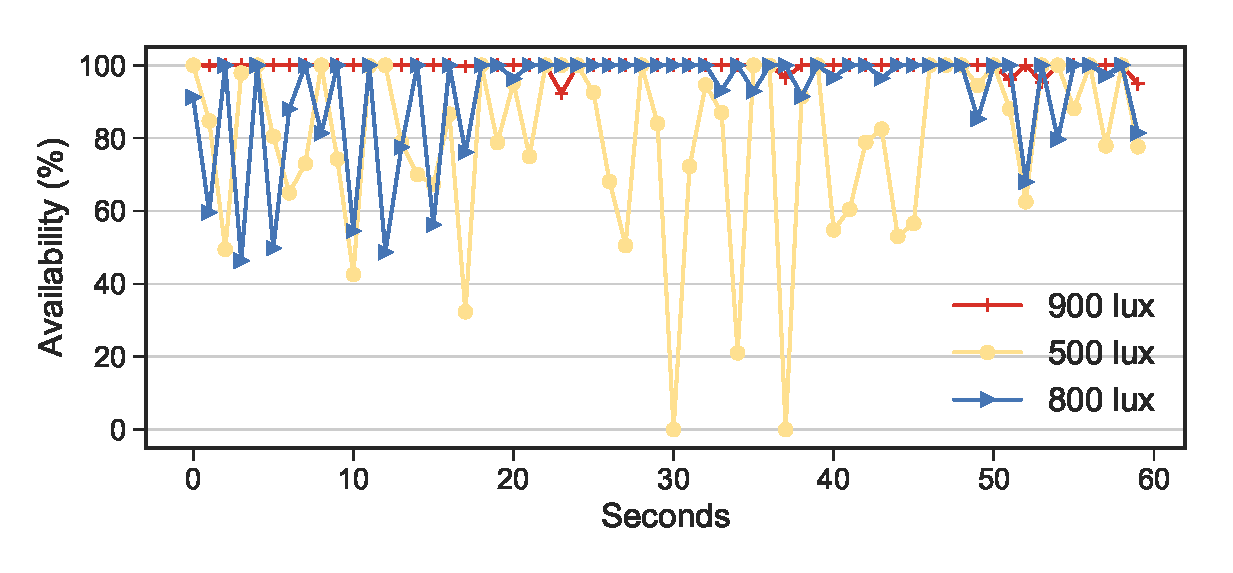
\includegraphics[width=\columnwidth]{figures/sysAvailabilityTimeline_470_sleep_5seconds_2}
    \caption{\cis availability observed with a 5 seconds time window.}
    \label{fig:fineScaleAvailability}
\end{figure}
% In Section~\ref{subSec:availability}, we discussed that the \cis availability is not a constant value. 
Since the nodes' on-times are in a constant shift relative to each other (Section~\ref{subSec:availability}), the collective availability of the \cis fluctuates when it is observed in a short time window. 
Figure~\ref{fig:fineScaleAvailability} captures \cis availability on a time window of 5 seconds for thee different ambient energy conditions. In these experiments, the average power cycles of the \cis's nodes are (3,18), (3.9,12.3), and (4.3,11.5) seconds when ambient light intensity are 500, 800, and 900\,$\si{lux}$, respectively. 
If we focus on the line graphs associated with 500 and 800\,$\si{lux}$ and compare the system availability within the interval $[20,50]$ seconds and the rest, we can observe that the \cis gradually alternates between low and high collective availability; nodes' on-times gradually transition from maximum to minimum separation and vice versa (Section~\ref{subSec:availability}). Notice that, when ambient light intensity was 800\,$\si{lux}$ the \cis collective availability transited from low to high to low, while this pattern happened to be reversed when light intensity was  500\,$\si{lux}$. For the 900\,$\si{lux}$ the 8-node \cis achieved near-continuous $100\%$ availability. 
%
% \begin{table}
%     \centering
%     \caption{The \cis availability on fine scale: the effect of the energy buffer size and the time interval within a \cis is observed on the system availability}
%     \label{tab:availFineScale}
%     \begin{tabular}{r|l|l|l|r}
%     \hline
%     Intervals (sec) & -    & RF ($47\si{\mu F}$)      & -    & light ($470\si{\mu F}$)  \\ 
%     \hline
%     -             & mean  & std     & mean     & std   \\ \hline
%     0.5             & 61    & 8.8     & 27.3     & 42.9   \\
%     1               & 61    & 5.9     & 27.3     & 41.5   \\
%     2               & 61    & 4.4     & 27.3     & 37.5   \\
%     \hline
%     \end{tabular}
% \end{table}

% Table~\ref{tab:availFineScale} captures the \cis availability on fine scale. An obvious but important observation is that the \cis availability flactuates, see the std columns.    for two different energy buffer sizes. 


% \begin{table}
%     \centering
%     \caption{The \cis availability on fine scale: the effect of the energy buffer size and the time interval within a \cis is observed on the system availability}
%     \label{tab:availFineScale}
%     \begin{tabular}{r|l|l|l|r}
%     \hline
%     Energy Intensity & -    & RF ($47\si{\mu F}$)      & -    & light ($470\si{\mu F}$)  \\ 
%     \hline
%     -             & mean  & std     & mean     & std   \\ \hline
%     high          & 61    & 8.8     & 91.3     & 24.9   \\
%     medium        & 43    & 7.4     & 67.6     & 44.3   \\
%     how           & 21    & 3.4     & 27.3     & 37.5   \\
%     \hline
%     \end{tabular}
% \end{table}




\subsection{Sensing}
\subsubsection{Experiment setup}
\label{sec:experiment_setup}
% \paragraph{availability on a fine scale}
 % \todo{Because of the differences in intermittent nodes power cycles, their duty cycles are constantly shifting relative to each other ( Figure~\ref{fig:cisOntime}).  However, this study does zoom in on the \cis availability on short time scale and the effect of length of the differences between the nodes power cycles on the system short term availability. } 
%
After validating our observation on different energy sources, we designed a testbed with controllable light intensity for clarity and reproducibility. To this end, we blocked uncontrollable light sources with a box of $60 \times 40 \times 40$\,cm. On the box ceiling, we attached a light strip of 2.5\,m with 150 LEDs that can produce 15 different light intensities. On the bottom a \fullCIM of 8 intermittent nodes is placed (see Section~\ref{sec:hardware} for hardware description).

The events in our experiments are spoken words (Table~\ref{tab:words}). 
Short events (see events classification in Section~\ref{sec:event_classification}) are represented with individual words, while burst events are represented with phrases of a few words.
We recorded different patterns of inter-event and inter-bust arriving time. We used a Bluetooth speaker~\cite{jbl} to replay a certain recording. 
% The data were collected using a logic analyzer~\cite{saleae} and processed on a laptop running Ubuntu 16.04 LTS. 
%
\subsubsection{Events detection rate}
%
\begin{figure}[t!]
		\centering
	    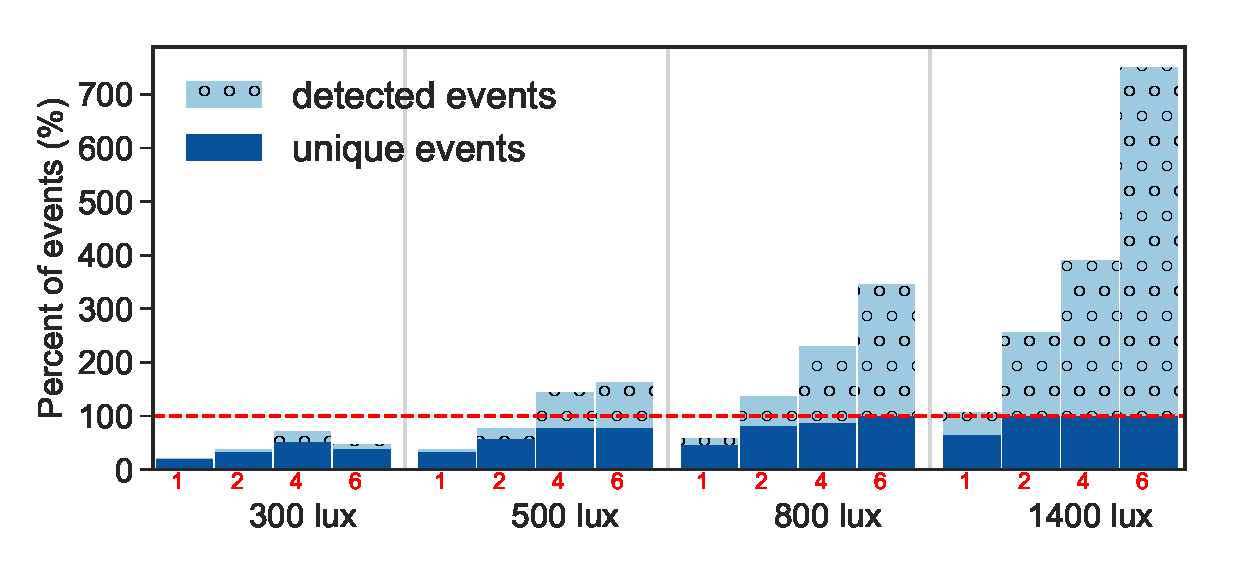
\includegraphics[width=\columnwidth]{figures/regular_events_capture_rate_2.eps}
		\caption{Duplicate and unique events captured by a \fullcim of eight solar-powered nodes. In general, the number of captured events increases in two case: when light intensity rises and when inter-event arrival time increases. 
         % In general, we see that when the light intensity increases, the number of detected and captured events rise too. Moreover, there is a positive correlation between the length of the inter-event arrival time and the detection and capture rates. 
         Red numbers indicate events arrival interval in seconds.
         }
    	\label{fig:events_detection_rate}
\end{figure} 
Here we experiment with the behavior of a \cis when events arrive individually or in bursts \emph{without} enabling  randomized response in favorable energy conditions. 
%
\begin{figure}[t]
    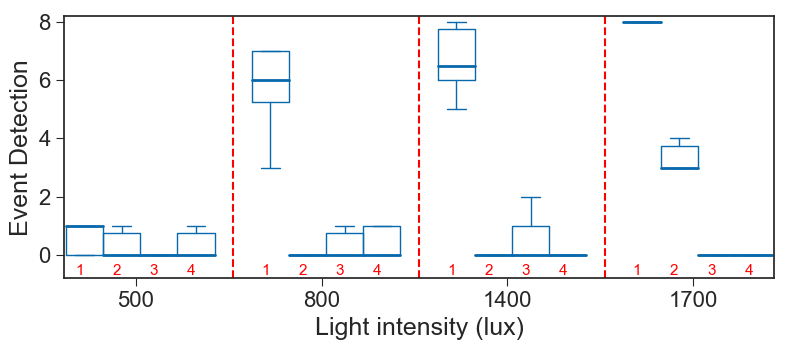
\includegraphics[width=\columnwidth]{figures/events_burst_problem_2}
	\caption{When capturing a burst of 4 events without randomizing the response, the majority of the nodes react to the first event in the burst and power down shortly after, missing the rest of the burst.}
    \label{fig:events_burst_problem}
\end{figure}
%
\paragraph{Individual events.}
\begin{figure}[t]
	\centering
     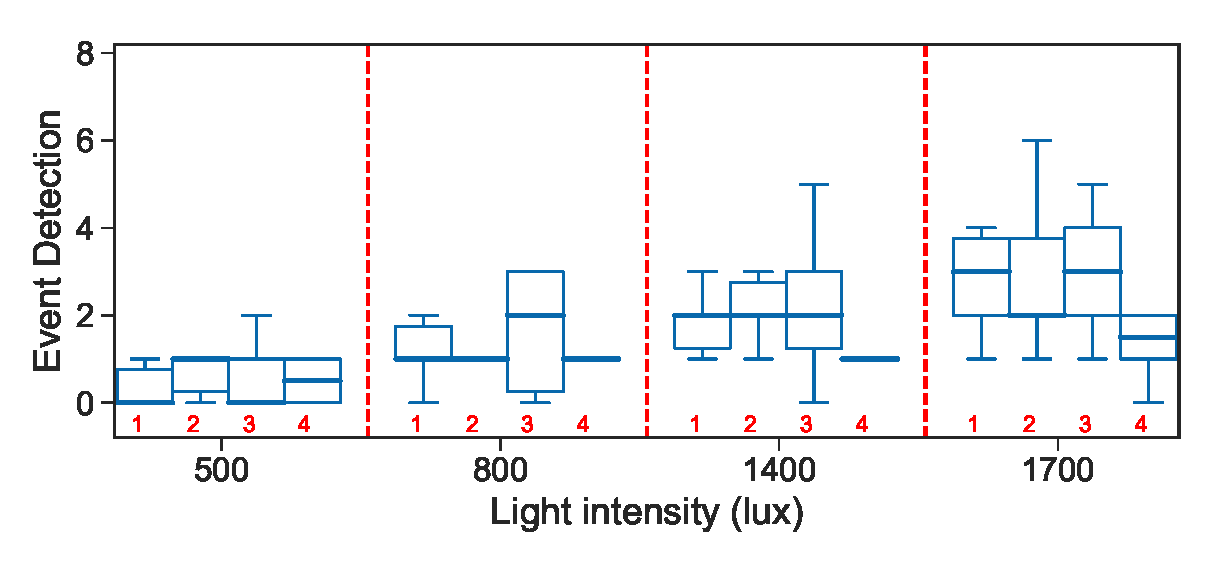
\includegraphics[width=\columnwidth]{figures/events_burst_rand_2}
    \caption{Response randomization enables a \cis to capture the entire burst of events with high capturing rates. It also reduces the number of duplicated events. Red numbers indicate events index in a burst.}
    \label{fig:events_burst_rand}
\end{figure}

Figure~\ref{fig:events_detection_rate} shows the percentages of capturing duplicate and unique events when light intensity varies from $\SI{300}{lux}$ to $\SI{1400}{lux}$ and the inter-event arrival time ranges from $\SI{1}{second}$ to $\SI{6}{seconds}$. For each experimental trial 20 words were played, resulting in a total of 240 playbacks. 

Figure~\ref{fig:events_detection_rate} shows a positive correlation between light intensity and the number of detected events. In particular, the number of duplicate detections rises dramatically when light intensity increases, \emph{demonstrating the overpowering problem} (Section~\ref{sec:power_state}). Moreover, increasing the inter-event arrival time also surges the number of duplicated events. The reason for this is that when the time between events increases, the intermittent nodes get the chance to sleep longer in low-power mode, consuming less energy. Thus, nodes' on-times expand, reducing their inherent randomization, which leads them to be in \textit{hibernating power state} (Section~\ref{it:hibernating}).  

% Indirectly, these results show how a \cis can achieve a much higher duty cycle than its individual intermittent nodes: Figure~\ref{fig:cis_nodes_dutyCycle} shows that with a light intensity of $\SI{800}{lux}$ an intermittent node is active with a duty cycle of 30\% while Figure~\ref{fig:events_detection_rate} shows that a \cis of 8 nodes captures 100\% of the unique events when the time between them is \SI{6}{s}. 

\textit{Bursty events.}
Figure~\ref{fig:events_burst_problem} shows the capturing behavior of a \cis when the events arrive in bursts. A burst of four events with one second between the individual events was fired every 20 seconds. Each burst was repeated 10 times and under four different light intensities. The nodes sleep in a low-power mode when they finish processing an event, waiting for the next one. 

In general, we observe that in favorable energy conditions (above $\SI{500}{lux}$) intermittent nodes react to the first event of a burst and power down shortly after, missing the rest of the burst. These results confirm our argument about the side effect of the \textit{hibernating power state} of a \cis (Section~\ref{sec:power_state}). These results also demonstrate that the hibernating power problem happens on a wide range of power intensities, showing its significance. Next, we will show how randomizing the response can mitigate the problems generated when ambient energy exceeds the design point. 

\subsubsection{Events detection rate with randomization}
\begin{table}
	\centering
    $
    \begin{array}{llll}\hline
     \textbf{(lux,second)} & \textbf{(800,6)} & \textbf{(1400,4)} & \textbf{(1400,6)}\\\hline
    \textit{randomization}    & 205/432 &  236/675 & 223/493 \\
    \textit{no randomization} & 240/831 &  240/938 & 240/1802 \\\hline
    \end{array}
    $
    \caption{These results are presented as \textit{unique/total} detected events. A node response probability is 65\% in the first two scenarios,\textbf{(800,6)} and \textbf{(1400,4)}, and 30\% in the last one.   
    Randomizing the response reduces the number of duplicated events by 50\% while losing only 7\% of the unique events.}
    \label{tab:regular_rand}
\end{table}
% 
Here, we examine the effect of enabling artificial randomization on the \cis's response. 

\paragraph{Individual events.} 
Table~\ref{tab:regular_rand} compares the number of detected events when the \cim's response is randomized and not randomized.
When randomization is enabled, nodes respond to events with a probability of 65\% for the scenario of $\left(\SI{800}{lux}, \SI{6}{seconds}\right)$ and $\left(\SI{1400}{lux}, \SI{4}{seconds}\right)$, and for the highest energy level and the longest inter-event arrival time the responding probability was set to 30\%.

Table~\ref{tab:regular_rand} shows that randomizing the response reduces duplicated events by an average of $\approx$50\%, while only marginally lowers the number of the uniquely detected events (7\% on average). 


\paragraph{Bursty events.}
To enable a \cis to capture events arrive in bursts, the response probability for each events in a burst should be different. The \cis should respond with a minimum probability to the first event in a burst and gradually increase the response probability for the subsequent events in the burst (we assume that between the bursts the \cis resumes to its expected collective availability). This gradual increment to the responding probability is motivated by the observation that when a node captures an event it becomes unavailable for the subsequent ones in the burst.
In this experiment, the nodes reacted with a probability of 40\%, 50\%, 70\% and, 100\% on the first, second, third and fourth event, respectively. Since the event distribution is known these probabilities were fixed during the development stage.

Figure~\ref{fig:events_burst_rand} shows how randomizing the \cis response spreads the nodes' awake times--as compared to Figure~\ref{fig:events_burst_problem}--and enables the \cis to capture the entire burst with a high probability, i.e., above 85\%. 
% Additionally, we also observe a positive impact of randomizing the response when the system is under-powered ($\SI{500}{lux}$).

%40 50 70 100


% \subsection{Coalesced intermittent command recognizer word detection accuracy}
% For evaluating the \fullcim accuracy, we used the word set in Table~\ref{tab:words}.
% Each word was pronounced by a single speaker 20 times and recorded on a PC. One of these recordings was stored as a template on the \cim, while the remaining 19 were played back through a Bluetooth speaker~\cite{microphone} for testing.

% The ratio between detected events and successfully recognized events per node is shown in Figure~\ref{fig:word_freq} and it averages out at  76.7\%. The difference between detection and capture is primarily caused by nodes that have insufficient buffered energy to finish recording.  

% %
% \begin{figure}
% \centering
% 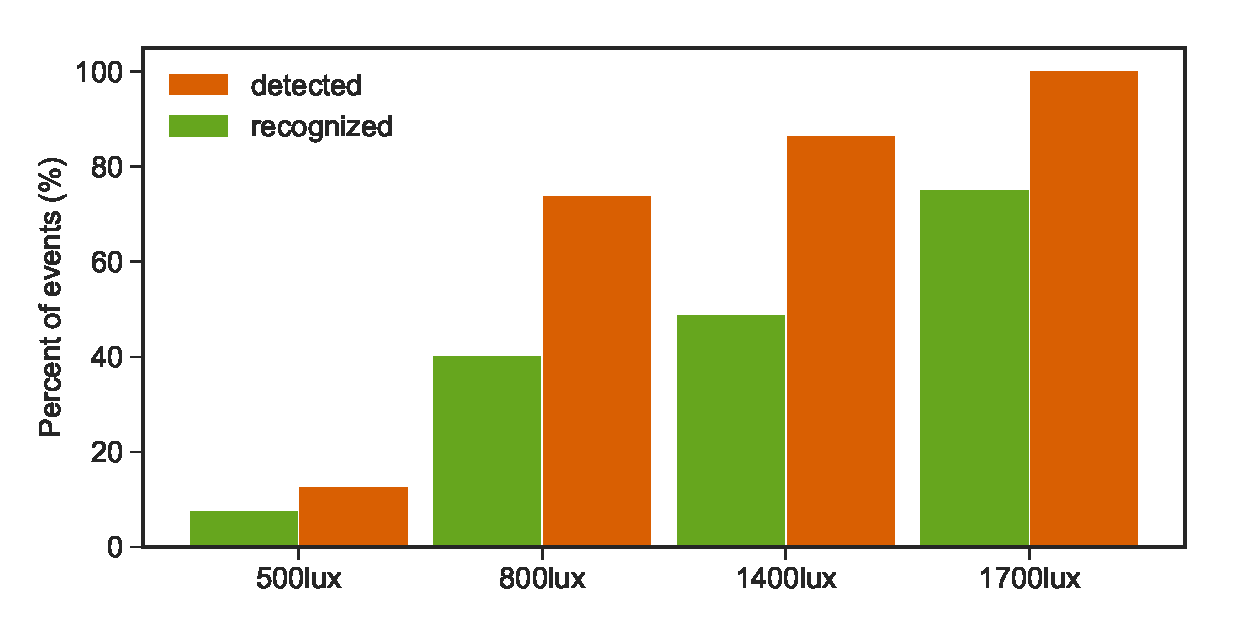
\includegraphics[width=\linewidth]{figures/detection_vs_recognition}
% \caption{
% % The percentage of successfully recognized words as compared to the detected ones.
% The average number of successfully recognized words per node and average number of detected words per node, as percentages of the total number of played words. Words are relatively long events and therefore some of their recordings do not complete due to insufficient harvested energy.}
% \label{fig:word_freq}
% \end{figure}

\begin{figure}
    \begin{subfigure}{0.48\columnwidth}
        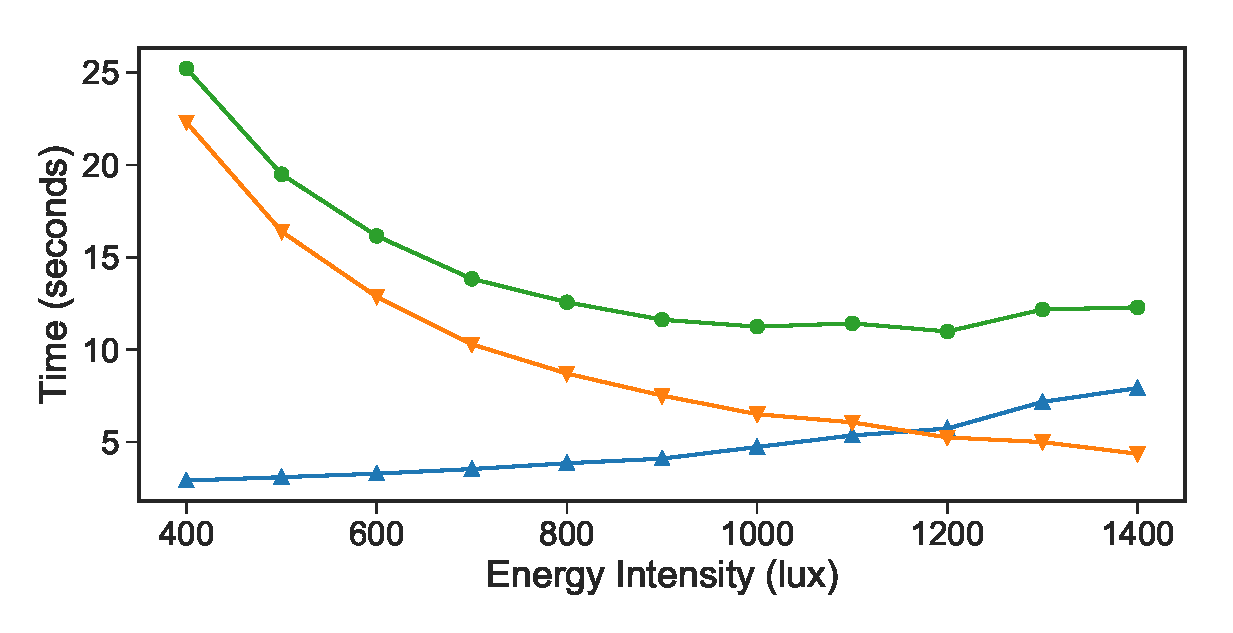
\includegraphics[width=\textwidth]{figures/BatterylessNodesDutyCycles_Sleep_mode}
        \caption{In wake-on-event style of operation, nodes go into low-power mode upon their power-ups. The low power consumption rate at this mode make the on-time of a node an important factor in determining the duty cycle and the power cycle length of the node.}
        \label{fig:differentEnergyIntensity}
    \end{subfigure}\hfill
    %
    \begin{subfigure}{0.48\columnwidth}
        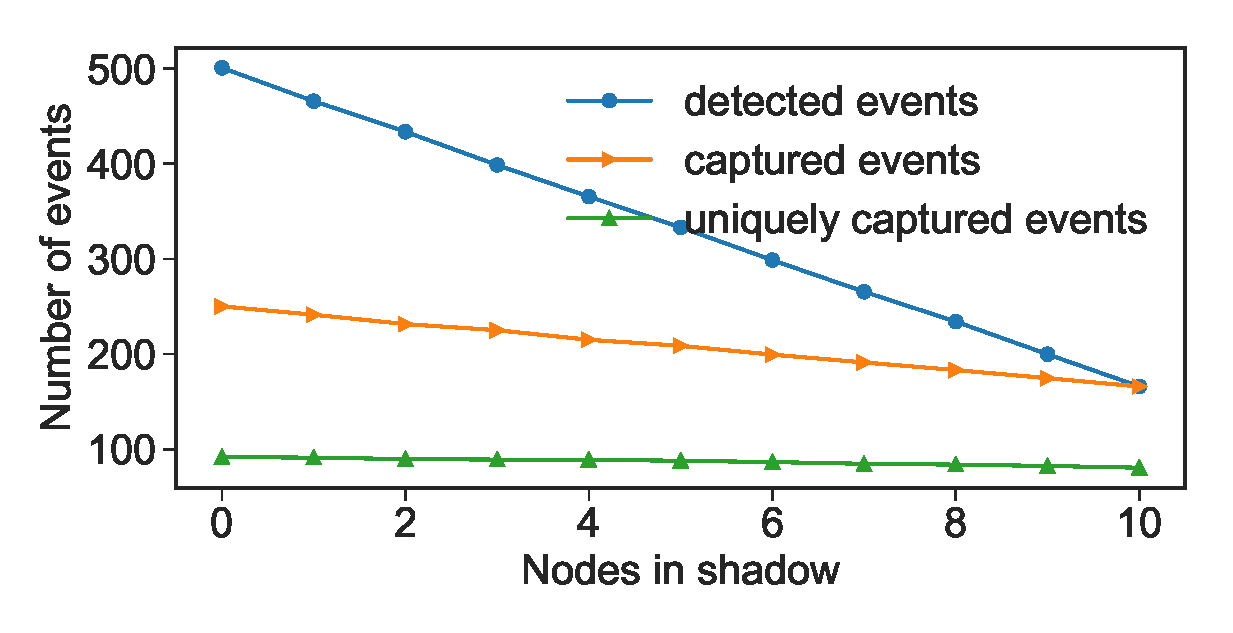
\includegraphics[width=\textwidth]{figures/different_energy_intensity}
        \caption{Simulated results showing how the number of captured events is affected when the shadow is covering a \cis. Detected events are \#times events trigger nodes. Captured events are \#times nodes processed events. We used a redundant factor of 2.5 (see (\ref{eq:randFactor})).}
        \label{fig:sim:differentEnergyIntensity}
    \end{subfigure}
    \vspace{-0.3cm}
    \caption{The effect of non-uniform energy distribution.}
    \label{fig:pwrCycleVSEnergyIntensity}
\end{figure}

\paragraph{Different energy harvesting rates}
It can happen that some of the nodes of a \cis are in the shadow while the rest is under direct sunlight (e.g., when curtains are being opened). 
As a consequence, nodes' power cycles will be significantly different (Figure~\ref{fig:differentEnergyIntensity} shows the on-times, off-times, and power cycles when the ambient energy ranges from 400 to 1400\,lux). Therefore, nodes will not be able to accurately estimate the collective availability of the system. 
%
The inaccurate estimation is most significant when half of the nodes are in shadow. 
However, even during such a worst-case scenario, a \cis availability is not dramatically effected (Figure~\ref{fig:sim:differentEnergyIntensity}). 
This is because half of the nodes will overestimate the availability of the system while the other half will underestimate the \cis's availability.
For example, in these simulation results the node with 50\% duty cycle responded to $\approx$\,50\% of the events while nodes with 16\% duty cycle responded with a probability of 100\%. 
During this simulation, the power cycles, on-time, and off-time of the nodes are 10, 5, and 5 units of time when they are under sunlight and 24, 4, and 20 when they are in shadow. 
The length of the simulated experiment is 1000 units of time and We used a redundant factor of 2.5 (see (\ref{eq:randFactor})).











































\section{Background}
\label{sec:background}
Here a minimal amount of background information is presented to facilitate clarifying the technical sections of the paper. 

\subsection{Energy-harvesting Devices}

%1. why \textit{small form factors EH sensor nodes}\\
Small sensors are less intrusive devices, and therefore, many applications prefer them on the bigger ones 
% (imagine the difference in the implications of embedding a sensor of the size of 2 AAA batteries and a sensor of a few cubic millimeters in volume in a shoe for step counting).  
%
Long sensors lifetime is also desirable. However, long sensors lifetime and small form factors are conflict goals.
% 2. classify EH with continuous power and tiny EH with intermittent power \\
For example, rechargeable batteries paired with energy harvesters can continuously power sensor nodes for relatively long time. But, rechargeable batteries inherent normal batteries drawbacks including increasing the size and limiting the sensor lifetime (although much longer) as rechargeable batteries typically wear out after a few hundreds charging cycles~\cite{}.
%
However, if an application's requirements put hard constraints on the size of the sensors, then removing the batteries is one of the first options to be considered. 
Battery-less energy-harvesting sensors operate intermittently. They charge a small capacitor to ensure uninterrupted operations for a minimum certain duration. Once, the capacitor has been depleted, the sensor powers down, letting the energy-harvester to accumulate energy again. 
%
Intermittent operation raises many challenges such as how to enable applications to span their execution over power failure~\cite{}, and how to enable timeliness operations when the durations of the device power-downs are indeterminate~\cite{}.
%
Big capacitors may allow longer operational periods of time, but they also need more time to charge. 
In order for a capacitor to charge, the input voltage must be higher than the accumulated voltage in the capacitor. 
This phenomena makes charging big capacitors using tiny energy harvester less efficient~\cite{}. 
boosting ambient energy using an energy-conditioning circuit is possible on the expense of device complexity, form factor, energy consumption, and cost. 

\subsection {Speech types}
%
Speech recognition algorithms can be classified based on the type of speech that they can recognize into \textit{spontaneous speech, continuous speech, connected word,} and \textit{isolated word}~\cite{gaikwad2010review}.
Systems with \textit{continuous} or \textit{spontaneous speech} recognition are the closest to natural speech, but are the most difficult to create because they need special methods to detect words boundaries~\cite{gaikwad2010review}. This is less the case for the \textit{connected word} type, where a minimum pause between the words is required.
 The type with the least complexity is the \textit{isolated word} type. It requires a period of silence on both sides of a spoken word and accepts only single words. 
 
Voice is a natural way for the human to interact with small devices. However,
implementing speech recognition on resources---memory, computation power, and energy---limited platforms is challenging, to say the least. Therefore, we attempt to recognize, with our command recognizer prototype, the simplest type of speech, isolated words. 

\section{Related Work}
\label{sec:relatedWork}
Recent advances in ultra-low-power microcontrollers along with the development of energy harvesters have enabled the creation of stand-alone battery-free sensors. These sensors operate intermittently because the power that they harvest is
weak and volatile.

\subsection{Energy-harvesting systems}
Energy harvesters have the potential to power devices indefinitely as they collect energy from perpetual energy sources. Sunlight, vibration, and radio frequency (RF) waves are examples of such energy sources. The power harvested from these sources vary wildly, for example, RF harvestable power ranges from
\si{\nano\watt}-scale when harvested from ambient signals to \si{\uW}-scale when collected from a dedicated RF signal emitter, and solar power varies from tens of \si{\uW} to tens of \si{\mW} when it is harvested by a solar panel of a few \si{\cm^2} illumination surface~\cite{lucia2017intermittent,rao2017ambient}.

Many battery-less energy-harvesting platforms have been proposed. Some of them
rely on dedicated external energy sources such as WISP -and its variants-, a
general wireless sensing and identification
platform~\cite{smith2006wirelessly,zhao2015nfc,zhang2011moo}; WISPcam,  an
RF-powered camera~\cite{naderiparizi2015wispcam} and, the battery-free
cellphone~\cite{talla2017battery}. Others, harvest from ambient sources such as
the ambient backscatter tag~\cite{liu2013ambient}, and the solar-powered
tag~\cite{majid2019multi}. Platforms that facilitate the development of
battery-less energy-harvesting systems have also been proposed. For instance,
Flicker~\cite{hester2017flicker}, a prototyping platform for battery-less devices; EDB~\cite{colin2016energy} an energy-interference-free debugger for intermittent devices;  and Capybara~\cite{colin2018reconfigurable}, a re-configurable energy storage architecture for energy-harvesting devices.

However, \emph{there is no energy-harvesting platform that considers the abstraction of many intermittent sensors (or nodes) and exploits the statistical energy harvesting differences between them to provide reliable sensing}.
% The paper is the first that considers the abstraction of a group of intermittent nodes and investigates the emerging collective duty cycle of the system. 
%experience. 

\subsection{Intermittent execution}
% What is the problem that requires intermittent execution
Intermittent execution models enable applications to progress despite frequent
power failures~\cite{van2016intermittent,colin2016chain,lucia2015simpler,bhatti2017harvos,gobieski2019intelligence}. To this end, they decompose an application into several small pieces and save the state of the computation on the transitions between these code segments. Therefore, intermittent applications do not return to the beginning of the program (i.e., \texttt{main()}) after each power failure.
%(in contrast to  applications that assume continuous power).
Instead, they resume execution from the last successfully saved progress state.   

% Sleep not to die 
% Intermittent systems are regarded as the successor of energy-aware systems. Dewdrop~\cite{buettner2011dewdrop} is an energy-aware runtime for (Computational) RFIDs such as WISP. Before executing a task, it goes into low-power mode until sufficient energy is accumulated. QuarkOS~\cite{zhang2013quarkos} divides the given task (i.e., sending a message) into small segments and sleeps after finishing a segment for energy recharge. However, these systems are not power disruption tolerant. In other words, if a system could not sustain the energy consumption of low-power mode and powers down, then all the computation progress will be lost. 

% checkpointing 
Mementos~\cite{ransford2011mementos} proposed a volatile memory \emph{checkpoint-based} approach to enable long-running applications on intermittently powered devices. DINO~\cite{dino} enables safe non-volatile memory access despite power failures. Chain~\cite{colin2016chain} minimizes the amount of data needed to be protected by introducing the concepts of \emph{atomic tasks and data-channels}. Hibernus~\cite{balsamo2014hibernus,balsamo2016hibernus++} measures the voltage level in the energy buffer to reduce the number of checkpoints per power cycle. Ratchet~\cite{van2016intermittent} uses compiler analysis to eliminate the need for programmer intervention or hardware support. HarvOS~\cite{bhatti2017harvos} uses both compiler and hardware support to optimize checkpoint placement and energy consumption. Mayfly~\cite{hester2017timely} enables time-aware intermittent computing. InK~\cite{yildirim2018ink} introduces event-driven intermittent execution.  
\emph{For our prototype implementation we adopt a power failure protection approach similar to that of DINO~\cite{dino}, see Section~\ref{sec:software}.}


\subsection{Speech recognition}
%  Speech recognition consists of several steps. The basic steps are:
% \textit{Speech recording and signal digitization}---a microphone records the sound waves and an ADC converts the microphone signal into a digital signal. A sampling rate of about 8 kHz is required to capture the frequencies of a human voice (100-4000Hz \cite{Bernal-Ruiz2005MicrocontrollerSystems}). \textit{Framing}---after that the digitized signal is divided into blocks of usually 10-30 ms~\cite{gaikwad2010review,delaney2002low,delaney2005energy} called frames. \textit{Features extraction}---for each frame a feature vector is extracted containing all the relevant acoustic information. \textit{Feature matching}---finally the extracted features are matched against features known to the recognizer. 

The speech recognition problem has been tackled from many angles and has experienced many breakthroughs. For example, the dynamic time warping (DTW) algorithm enables matching voice signals with different speed (or time) \cite{vintsyuk1968speech}. 
Approaches based on Hidden Markov Models showed much better performance than DTW-based ones~\cite{jelinek1997statistical}. Hence, they became the standard techniques for general-purpose speech recognition until artificial intelligent algorithms~\cite{hinton2012deep} outperform them. 
% Furthermore, many specialized hardware architectures for speech recognition have been proposed to, for instance, reduce energy consumption \cite{price2018low,price20156}. 

% The evolvement of the speech recognition algorithms has enabled them to recognize more complicated type of speech. 
% From a recognition algorithm perspective the speech can be classified
% Speech recognition algorithms can be classified based on the type of speech that they can recognize 
From a recognition complexity standpoint, we can classify the speech into \textit{spontaneous speech, continuous speech, connected word,} and \textit{isolated word}~\cite{gaikwad2010review}.
The \textit{continuous} and \textit{spontaneous speech} are the closest to natural speech, but they are the most difficult to recognize because they need special methods to detect words boundaries~\cite{gaikwad2010review}. This is less the case for the \textit{connected word} type, where a minimum pause between the words is required. The type with the least complexity is the \textit{isolated word}, as it requires a period of silence on both sides of a spoken word. 
 
% Voice is a natural way for the human to interact with small devices. However, 
Speech recognition on resources---memory, computation power, and energy---limited platforms is challenging, to say the least. Therefore, \emph{our command recognizer targets isolated-word type of speech}. 





















\section{Discussion and Future Work}
\label{sec:discussion}

\section{Conclusion}
Energy-harvesting battery-less sensors can operate very long because their power source is unlimited. 
However, ambient power is weak and volatile; therefore, these sensors operate intermittently.
The intermittent availability compromises their value as they have a high probability of missing events. 
This paper addresses the \emph{availability} problem of intermittent sensors. 
%
It presents the \textit{\fullcis} (\cis), which is the abstraction of a group of intermittently-powered sensors.
A \cis is able to approach continuous sensing by taking advantage of the embedded randomization in the powering subsystem of intermittent sensors.
The resulting differences in the sensor nodes' power cycles make the nodes' on-times uniformly distrusted. 
Therefore, the number of a \cis nodes can be seen as a design parameter to achieve a targeted collective availability. 
% Therefore, adding more nodes to a \cis increases its expected availability. 
We have modeled the availability of a \cis and its effective availability: the availability that leads to successful event capturing. 
Further, we showed the accuracy of these models by validating them against data collected on real hardware and with different ambient energy sources (i.e., sunlight, artificial light, and RF). 
%
Furthermore, we showed how the variation in nodes' power consumption and harvesting rate and the arrival of external events can compromise the \cis's availability (nodes employing sleeping mode to increase the chance of successfully capturing an event, synchronize their power cycles on the first incoming event, in a burst, and miss the subsequent ones. The probability of this unwanted synchronization increases when ambient energy rises beyond the design point.  
% It taking advantage of the embedded randomization in the powering subsystem of energy-harvesting battery-less sensors to distribute
% the on-times of a group of intermittent sensors uniformly in time 
% We presented the \textit{\fullcis} (\cis), an intermittently powered ``sensor'' that senses continuously! \cis is built around the observation that multiple intermittent nodes distribute themselves uniformly in time. This observation enables us to accurately model, and validate on real hardware, the \cis availability---the collective on-time of its intermittent nodes. 
% An important finding is that favorable energy conditions may cause sleeping intermittent nodes to synchronize their power cycles on the arrival of the first event. Consequently, they react to the same event, start recharging at the same time, and missing the next event. 
% 
To counter this unwanted behavior, we designed an algorithm to estimate the number of active neighbors and respond proportionally to an event. 
We developed a prototype of the \cis, an 8-nodes \fullCIM (\cim). 
Using this prototype, we showed that the \fullcis is able to distribute bursts of events on its nodes "evenly" and capture the entire burst with above 85\% detection accuracy.
 

Intermittent sensors will partially capture events. Classical algorithms for recognizing and classifying these events might face difficulties  dealing with partially captured data. Thus, follow-up work can investigate \emph{how much machine learning algorithms can improve the sensing quality of intermittent sensing?} 
% Additionally, the command recognition rate could further be improved by using an estimation of the energy left in the energy buffer, to start recharging early. This will prevent a detection when there is not enough harvested energy to record for a long enough time, letting a node recharge earlier and coming back with sufficient energy.


% \noindent\textbf{Speech Recognition on Intermittent Devices} In this paper, we have shown the feasibility of speech recognition on intermittent power. We also demonstrated the possibility of recognizing burst of events (in our case four words). However, the type of speech we targeted is the simplest, isolated words. Next, we may attempt recognizing a more complicated type of speech and for a larger number of words than the number chosen for this study.



%comment it out before submitting
\newpage

\bibliographystyle{ACM-Reference-Format}
\bibliography{references}

\end{document}
